\nenwin can simulate a single-bit register (i.e. an off-on memory cell).
We present an architecture, for which we can prove the following properties:
\begin{enumerate}
    \item It is possible to read the 0 state
    \item It is possible to read the 1 state
    \item It is possible to set the bit to 0
    \item It is possible to set the bit to 1
\end{enumerate}
The register will be operated by sending a Marble to one of 3 (there is one for reading, one for writing and one for erasing the bit) MarbleEmitterNodes at the edge of the bit. The output will result in a Marble occurring at one of two specific locations that depend on the bit state. This Marble could from there be redirected, or be consumed by a MarbleEaterNode. In the provided architecture the '0-reader' and the '1-reader' are MarbleEaterNodes used at these locations, but for different purposes different elements could be placed here.

\subsubsection{Architecture}
We define the bit architecture $\B$, implemented in $\mathbb{R}^3$ as follows:
\begin{itemize}
    \item Let $P$ be a two-dimensional hyperplane in $\mathbb{R}^3$.
    \item At a specific position in $P$, we create the center of the bit (the 'bit-position'): in the '1' state, this position is occupied by a specific 'bit-Marble', but empty in the '0' state.
    \item A 'bit-emitter' MarbleEmitterNode is placed along the line $l$, which runs though the bit position orthogonal to $P$. We give this MarbleEmitterNode a radius such that the edge of the radius is an infinitesimal distance from the bit position. The Marble that it can emit is the bit-Marble at the bit position.
    \item A 'signal-emitter' MarbleEmitterNode, that is placed at a distance from the bit position in $P$, with a radius sufficiently small not to contain the bit position. The threshold distance is also smaller than the distance from this signal-emitter to the bit-position.
    \item A 'signal-Marble' that can be emitted by the signal-emitter. This Marble has a positive velocity in the direction from the signal-emitter toward the bit-emitter, and is used to pass an external 'write'-signal received by the signal-emitter to the bit-emitter. It has the same mass as the bit-Marble.
    \item Let $\varepsilon \in \mathbb{R}$ be a small yet finite positive number.
    \item A 'read-emitter' MarbleEmitterNode, that is like the signal-emitter also placed in $P$ with a radius and a threshold sufficiently small not to interfere with the bit position. However, it is placed on a different position than the signal-emitter. 
    \item A '0-reader' MarbleEaterNode that is placed in $P$ on the opposite side of the bit position as the read-emitter, but such that the line between the 0-reader and the read-emitter is a distance $\varepsilon$ from the bit position. The radius of this Node can be small but nonzero, and the threshold distance of its attraction is set to 0.
    \item A 'read-Marble' that can be emitted by the read-emitter, that has an opposite side as the bit-Marble (and hence is repelled by the bit), and a Marble-stiffness of 0. It has a velocity vector in the direction from the read-emitter towards the 0-reader.
    \item A '1-reader' MarbleEaterNode, that is placed in $P$ at an equal distance from the bit-position as the '0-reader', but located such that it will catch the read-Marble if it is repelled by the bit-Marble: it will be proven below that this is not the same location as that of the 0-reader. The radius and the threshold distance have the same values as in the 0-reader.
    \item An 'eraser-emitter' MarbleEmitterNode, similar to the signal-emitter, but at a different position. 
    \item A 'garbage-collector' MarbleEaterNode with similar properties as the 0-reader and the 1-reader, but located exactly on the line running from the eraser-emitter to the bit-position, on the opposite side of the bit-position as the eraser-emitter (this is also in $P$). This Node solely functions to delete Marbles.
    \item An 'eraser-Marble' that can be emitted from the eraser-emitter, with a velocity in the direction from the eraser-emitter towards the bit-position (and hence also towards the garbage-collector). The mass of this eraser-Marble will have the opposite sign as the bit-Marble, and it will have a Node- and Marble-stiffness of 1. The gravity threshold distance of this eraser-Marble is nonzero.
\end{itemize}

The Nodes defined above can all be placed in $\mathbb{R}^3$, on different positions while satisfying their description. All Nodes and Marbles defined above, except the bit-emitter, are placed in $P$ \footnote{It is also possible to place the bit-emitter in $P$, but this would lead to more complex proofs as we need to ensure that it will not interfere with any Marble moving though $P$.}. 

Note that $\B$ should be placed in a region of $\mathbb{R}^3$ where no external forces (except for the Marble that activates reading/writing/erasing) apply, and that when using the threshold gravity function \ref{eq:tresholdgrav}.

The particles of $\B$ and their important properties have been summarized in Table \ref{table:bit}.

\begin{table}[h]
    \begin{tabular}{l|l|l|l|l}
    \textbf{Particle} & \textbf{Type} & \textbf{Mass sign} & \textbf{Marble-stiffness} & \textbf{Marble-attraction} \\ \hline
    bit-Marble        & Marble            & - & 0 & 1 \\
    bit-emitter       & MarbleEmitterNode & 0 &   &   \\
    signal-emitter    & MarbleEmitterNode & 0 &   &   \\
    signal-Marble     & Marble            & - &   &   \\
    read-emitter      & MarbleEmitterNode & 0 &   &   \\
    0-reader          & MarbleEaterNode   & + &   &   \\
    reader-Marble     & Marble            & + & 0 & 0 \\
    1-reader          & MarbleEaterNode   & + &   &   \\
    eraser-emitter    & MarbleEmitterNode & 0 &   &   \\
    garbage-collector & MarbleEaterNode   & 0 &   &   \\
    eraser-Marble     & Marble            & + & 1 & 1
    \end{tabular}
    \caption{Summary of the particles in $\B$, with their most important attributes. 
    Irrelevant values have been omitted: the bit can be made to work for multiple values of these variables. For the mass only the sign and not the magnitude has been recorded, except where the mass is 0. Note that it may not be strictly required to make those particles mass-less, but it simplifies the proof.}
    \label{table:bit}
\end{table}


\begin{figure}
    \centering
    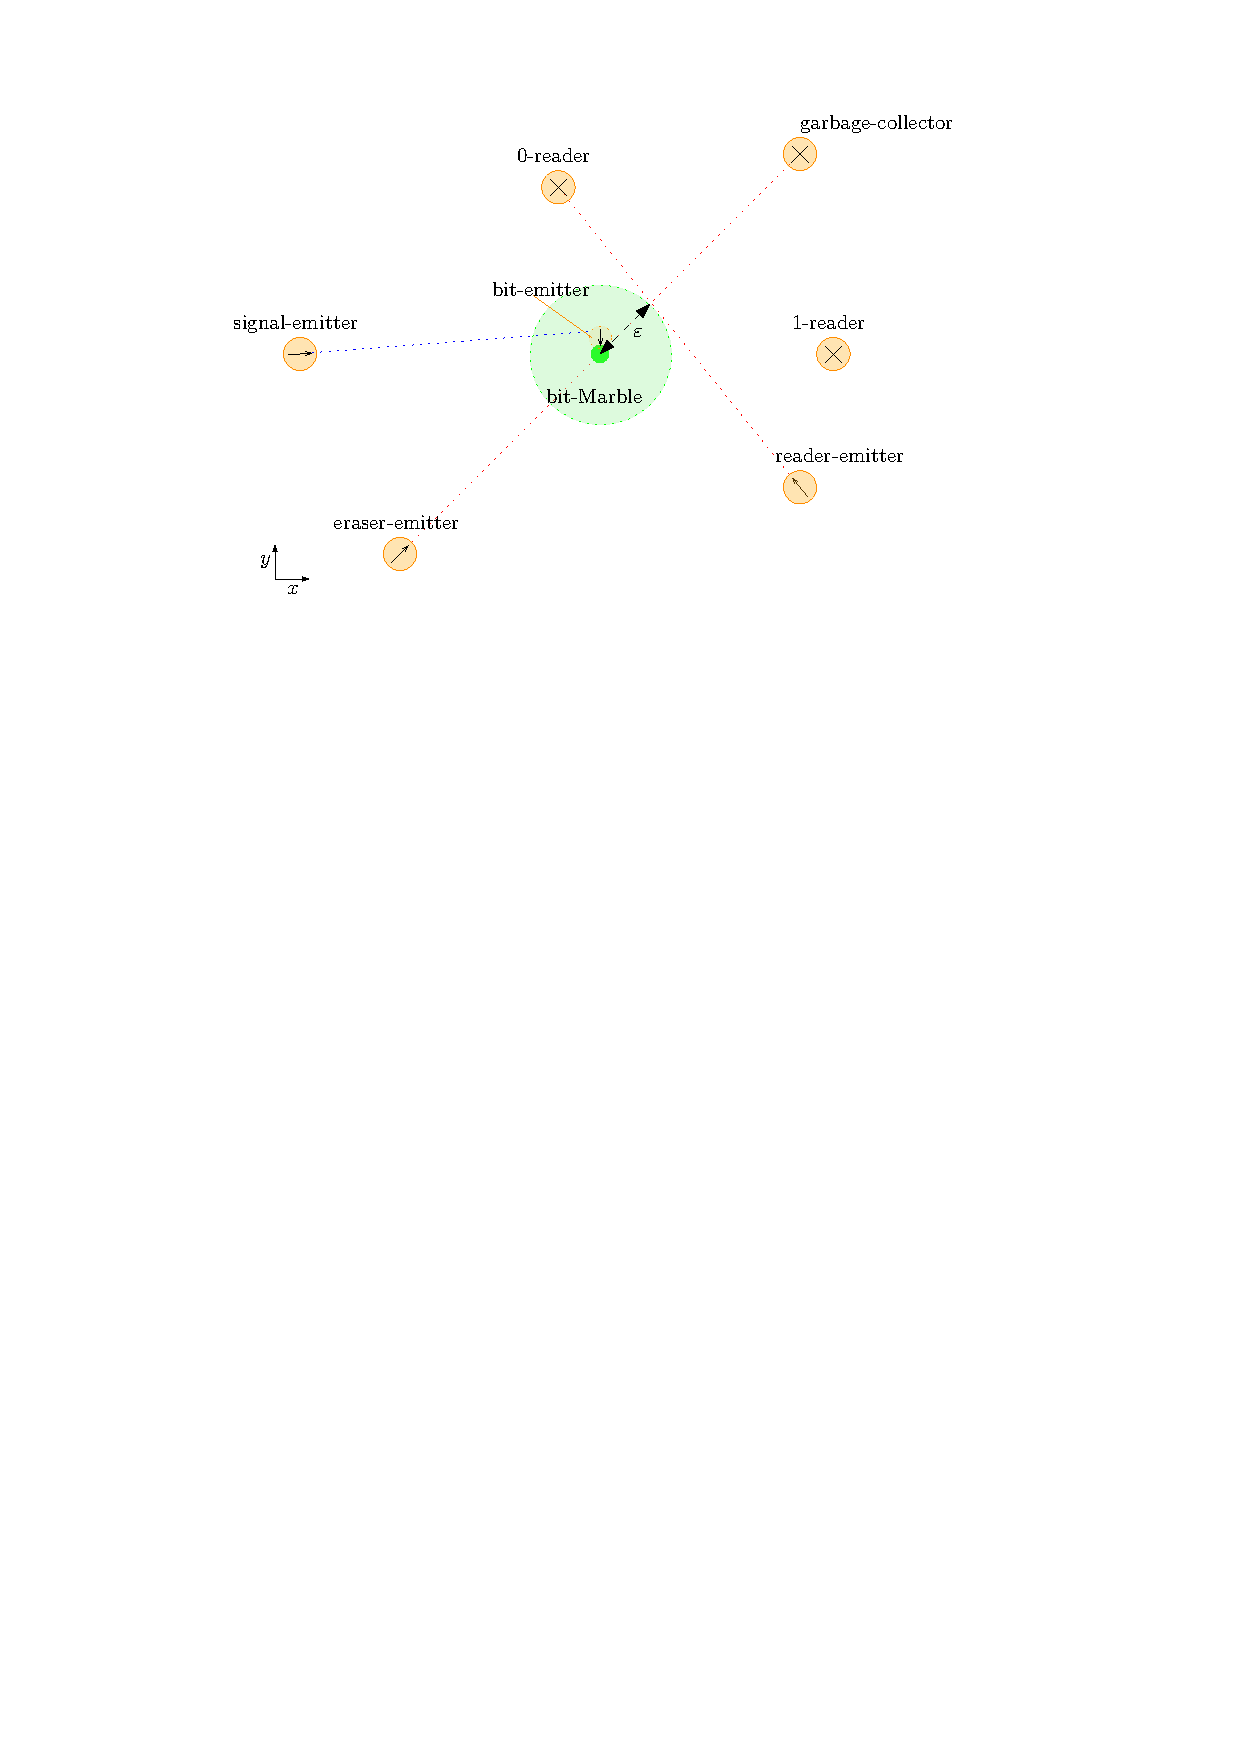
\includegraphics{figures/bit_base.pdf}
    \caption{A visualization of the bit-register architecture $\B$, as projected on a 2-dimensional image. 
    	The Bit-Marble is drawn in green, with the threshold-gravity-radius drawn in light-green. 
    	Note that the distances and sizes are not necessary to scale. Hypothetical paths of emitted Marbles are sketched with dotted lines (hypothetical in the sense that the emitted Marbles would follow this path if no forces acted on it).}
    \label{fig:bit_architecture}
\end{figure}

Let $\gamma \subseteq \mathbb{R}^3$ denote the smallest continuous cuboid region in $\mathbb{R}^3$ in which $\B$ has influence (i.e. all particles of $\B$ and all their attraction fields are contained in $\gamma$). 

\begin{lemma}[Reading state 0]
    An external Marble can trigger architecture $\B$ to increase the output of the 0-reader by 1 if the bit register is in the 0-state. After this operation, $\B$ will be in the same state as it started except for the value of the 0-reader.
    \label{lemma:0-reader}
\end{lemma}
\begin{proof}
    Consider an external Marble that enters $\gamma$ at the facet of $\gamma$ that is closest to the reader-emitter, 
    and let this Marble have velocity that moves it in a straight line to the reader-emitter. 
    If this Marble has the correct mass, then the reader-emitter will emit a reader-Marble. 
    This reader-Marble has an initial velocity in the direction of the 0-reader, by design of $\B$. 
    Since there is no bit-Marble to alter its course of motion (since the bit is in state 0) 
    nor any other attraction along its way, it will arrive at the 0-reader. 
    
    Note that the reader-Marble cannot intersect the radius of the bit-emitter, 
    since the bit-emitter does not intersect the plane $P$, in which the reader-Marble remains its entire existence 
    (it moves along the line from the reader-emitter to the 0-reader. These two Nodes are in $P$, and therefore this entire line is in $P$).
    
    Clearly, no particles that existed before the external Marble entered $\gamma$ have been changed during this operation, 
    except for the state of the 0-reader.
\end{proof}

\begin{lemma}[Reading state 1]
     There exists a location for the 1-reader, a value for $\varepsilon$, a mass value and a gravity threshold value for the bit-Marble, such that an external Marble can trigger architecture $\B$ to increase the output of the 1-reader by 1, if the bit register is in the 1-state. After this operation, $\B$ will be in the same state as it started except for the value of the 1-reader.
     \label{lemma:1-reader}
\end{lemma}
\begin{proof}
    As in Lemma \ref{lemma:0-reader}, an external Marble can cause the reader-emitter to emit a reader-Marble. Since the state of the bit is 1, there is a bit-Marble at the bit-position. Now we can adjust $\varepsilon$ and the threshold of the bit-Marble's gravity such that the path of the reader-Marble will intersect the attraction field of the bit-Marble at its boundary. Let $p$ the point where this boundary and the line between the reader-emitter and the 0-reader (which define $\varepsilon$) intersect. 
    
    The direction of movement the reader-Marble will not be altered form its starting velocity until it reaches point $p$. 
    At this point, only the acceleration of the reader-Marble will be affected. 
    This is true because the mass of the bit-Marble is, 
    by construction, of the opposite sign as that of the reader-Marble, 
    and because the reader-Marble does not attract Marbles while it is attracted by them (by construction).
    The reader-Marble will be accelerated in the same direction as the line segment between the bit-position and $p$, 
    and this direction is orthogonal to the direction of the reader-Marble's initial velocity. 
    
    Since the reader-Marble intersects only shortly this acceleration is present only one instant of time. 
    However, if the mass of the bit-Marble is of sufficient magnitude, 
    it will change the direction of the velocity of the reader-Marble significantly. 
    The new direction of this velocity is not the opposite of the original direction, 
    as the acceleration was orthogonal to the original velocity of the reader-Marble. 
    Hence the reader-Marble will not arrive at the reader-emitter 
    (which requires the opposite direction as the original velocity of the reader-Marble had) 
    nor the 0-reader (which requires the original direction). 
    
    Note that the reader-Marble cannot intersect the radius of the bit-emitter, 
    since the bit-emitter does not intersect the plane $P$, in which the reader-Marble remains its entire existence.
    (As in Lemma \ref{lemma:0-reader}, the entire path of the reader-Marble is in $P$. 
    Since $p$ is on the line between the reader-emitter and the 0-reader, $p$ is in $P$ as well. 
    Now since the bit-position is also in $P$, the acceleration vector is also in $P$. 
    The resulting velocity of the reader-Marble is a linear combination of its prior velocity and the acceleration, 
    which are both vectors in $P$, hence the reader-Marble remains in $P$.)
    
    The 1-reader can be positioned along the line from the reader-Marble in the new direction of the Marble's velocity, 
    and then the reader-Marble will eventually be consumed by the 1-reader.
\end{proof}

\begin{lemma}[Writing bit]
    An external Marble can trigger architecture $\B$ when in state 0 (no bit-Marble present) to enter state 1 (with a bit-Marble present), without any other particle in $\B$ being affected after completion.
    \label{lemma:writing}
\end{lemma}
\begin{proof}
    Let the external Marble enter $\gamma$ in the point closest point of the closest facet of $\gamma$ to the signal-emitter, with a velocity the direction of the line from that point to the signal-emitter. Then this Marble will be consumed by the signal-emitter, and if it of sufficient mass it will trigger the signal-emitter once to emit a signal-Marble.
    
    The signal-Marble is configured (by construction of $\B$ to have a velocity in the direction of the signal-emitter towards the bit-emitter, and since it is not attracted by Marbles or Nodes, nor does any Eater- or EmitterNode block its path, it will eventually be consumed by the bit-emitter. Consequently, the bit-emitter creates a single bit-Marble.
\end{proof}

\begin{lemma}[Erasing bit]
    An external Marble can trigger architecture $\B$ when in state 1 (a bit-Marble present) to enter state 1 (no bit-Marble present), without any other particle in $\B$ being affected after completion, except for the mass stored in the garbage-collector.
    \label{lemma:erasing}
\end{lemma}
\begin{proof}
    Let the external Marble enter $\gamma$ in the closest point of the closest facet to the eraser-emitter, with a velocity in the direction of the line from this point towards the eraser-emitter. The Marble will be consumed by the signal-emitter, and if the external Marble had enough mass, an eraser-Marble will be emitted in the direction of the bit position. Note that the eraser-Marble has both a Node- and Marble-stiffness of 1, hence no attraction force will affect its acceleration. Hence it will travel in a straight line with constant velocity.
    
    The eraser-Marble has a Marble-stiffness of 1, and since the bit-Marble has a Marble-stiffness of 0, the bit-Marble's motion will be affected when the eraser-Marble nears the bit-Marble. Since the mass of the eraser-Marble is of the opposite sign as that of the bit-Marble, it will repel the bit-Marble, which will be accelerated in the same direction as the eraser-Marble is moving. Now we can adjust the masses of the bit-Marble and the eraser-Marble such that the repellent force is strong enough the accelerate the bit-Marble to the same or a higher velocity as the eraser-Marble before the eraser-Marble reaches the bit-position: this will guarantee that the eraser-Marble will not 'take-over' the bit-Marble and repel it in the other direction.
    
    Now both Marbles will travel in the direction of the line from the eraser-emitter to the bit-position. By construction of $\B$, the garbage-collector is also on this line and on the other side of the bit-position as the eraser-emitter. Therefore both Marbles will eventually enter the radius of the garbage-collector and be absorbed.
\end{proof}

We can summarize the results of Lemma \ref{lemma:0-reader}, \ref{lemma:1-reader}, \ref{lemma:writing} and \ref{lemma:erasing} in the following theorem:

\begin{theorem}[Bit register]
    There exist settings for the parameters of $\B$, and an external Marble $m$ outside of $\gamma$, such that by moving $m$ with the right value of $m.vel$, $m.pos$ and $m.mass$ into $\gamma$:
    \begin{enumerate}
        \item $m$ can trigger the reading of the bit. That is, after sufficient time, if there is a bit-Marble present, the 1-reader's number-of-Marbles-consumed count will increase by 1. If there no bit-Marble present, after sufficient time, the count of the 0-reader will increase by 1. When this count increases, the collection of particles in $\gamma$ and their states are identical to the situation before $m$ entered $\gamma$.
        \item $m$ can cause the creation of a bit-Marble in $\B$ without affecting the state of other particles in $\B$.
        \item $m$ can cause the removal of a bit-Marble in $\B$, when present, without affecting the state of other particles in $\B$ except for the Marbles consumed by the garbage-collector.
        \item Furthermore, $\B$ does not directly affect particles outside $\gamma$.
    \end{enumerate}
\end{theorem}
\begin{proof}
    \begin{enumerate}
        \item Follows from Lemma \ref{lemma:0-reader} and Lemma \ref{lemma:1-reader}.
        \item Follows from Lemma \ref{lemma:writing}.
        \item Follows from Lemma \ref{lemma:erasing}.
        \item The particles in $\B$ are constructed around a finite distance from the bit-position in $\mathbb{R}^3$, use finite radii and are using the threshold gravity as attraction function with a finite threshold. Hence in each direction from the bit-position, there is a distance that surpasses the influence of attraction functions, radii and positions of particles. By construction of $\gamma$, the minimum value of this distance either defines a facet of $\gamma$ or is interior to $\gamma$. Hence outside $\gamma$, $\B$ cannot affect any particle directly.
    \end{enumerate}
\end{proof}